\documentclass[a4paper,11pt]{article}

\usepackage[T1]{fontenc}
\usepackage[utf8]{inputenc}
\usepackage[english]{babel}
\usepackage{microtype}
\usepackage{graphicx}
\usepackage{booktabs}
\usepackage{tabularx}
\usepackage{enumitem}
\usepackage{geometry}
\usepackage{xcolor}
\usepackage{xspace}
\usepackage{hyperref}

\geometry{left=32mm,right=32mm,top=30mm,bottom=32mm}
\graphicspath{{figures/}}
\setlength{\parindent}{0pt}
\setlength{\parskip}{0.72\baselineskip}
\setlist[itemize]{leftmargin=1.5em,itemsep=0.2em,topsep=0.2em}
\setlist[enumerate]{leftmargin=1.5em,itemsep=0.2em,topsep=0.2em}

\definecolor{gspblue}{HTML}{1F4E79}
\hypersetup{
  colorlinks=true,
  linkcolor=gspblue,
  urlcolor=gspblue,
  citecolor=gspblue,
  pdftitle={The Graphics Server Protocol},
  pdfauthor={Nicolas P. Rougier and Cyrille Rossant}
}

\newcommand{\gsp}{GSP\xspace}
\newcommand{\vispytwo}{VisPy2\xspace}
\newcommand{\datoviz}{Datoviz\xspace}
\newcommand{\matplotlib}{Matplotlib\xspace}

\title{\textbf{The Graphics Server Protocol}\\
\large A shared semantic rendering layer for scientific visualization}
\author{Nicolas P. Rougier \and Cyrille Rossant}
\date{Draft for discussion - July 2026}

\begin{document}
\maketitle

\begin{abstract}
Scientific visualization libraries expose many different user APIs, but they repeatedly solve the
same lower-level rendering problems: batching large numbers of primitives, mapping data to visual
attributes, maintaining interactive views, exporting publication figures, supporting remote or
headless execution, and adapting to heterogeneous graphics backends. This duplication is especially
costly when high-quality GPU rendering is required. The Graphics Server Protocol (\gsp) proposes a
shared protocol layer for scientific visualization: semantic enough to preserve the meaning of a
visual scene, explicit enough to support conformance testing and backend capability discovery, and
low-level enough to target fast local GPU rendering, reference CPU rendering, remote renderers, and
future web paths. This white paper describes the rationale for \gsp, its current design principles,
the role of semantic visual families, the importance of explicit capability negotiation and
query/readback, and the current reference implementation strategy built around \matplotlib,
\datoviz, and \vispytwo. It is not an API reference; it is an invitation to discuss the protocol
boundary that scientific visualization libraries could share.
\end{abstract}

\tableofcontents

\section{Motivation}

Scientific visualization has never had a shortage of plotting APIs. A researcher can choose a high
level grammar, a stateful plotting library, a domain-specific viewer, a 3D visualization toolkit, a
browser-based charting system, or a low-level GPU library. These projects differ in user experience,
language ecosystem, deployment target, and visual style. That diversity is valuable: no single user
API can cover the needs of static publication plots, interactive exploratory tools, microscopy
viewers, computational geometry, neural data inspection, volume rendering, and web dashboards.

The problem is lower in the stack. Underneath these different APIs, many libraries rebuild the same
renderer-facing concepts. They need to place points, markers, line segments, paths, images, text,
meshes, axes, colorbars, cameras, and interactive views. They need to map scalar data through color
scales. They need to express coordinate systems and transforms. They need to answer basic scientific
questions such as ``what item is under this cursor?'' or ``what data value is represented by this
pixel?'' They need publication-quality output in one context and fast GPU interaction in another.
They need to run locally, in notebooks, in CI, on remote machines, and eventually in browser or cloud
rendering contexts.

Today these concerns are usually packaged as inseparable products: a user API plus a scene model
plus a renderer plus an interaction system. Moving a visualization from one renderer to another
often means rewriting it. A library author who wants both \matplotlib-quality static output and
GPU-speed interaction must either maintain two paths or accept one set of trade-offs. A domain
viewer that wants remote rendering must invent its own protocol or adopt a full web stack. A GPU
renderer that wants broad adoption must design a full plotting API, even if its real strength is
rendering.

\gsp is a proposal to separate these layers. Its goal is not to replace plotting libraries. Its goal
is to define a protocol surface that different plotting libraries, domain libraries, and renderer
implementations can share.

\begin{quote}
\gsp is the layer below plotting APIs and above concrete rendering engines. It describes scientific
visual scenes, resources, views, queries, capabilities, and diagnostics in backend-independent
terms.
\end{quote}

That sentence is the center of the project. A protocol at this level should not decide whether a
user writes an object-oriented plotting call, a grammar of graphics, a declarative JSON document, or
a domain-specific viewer script. It should decide what semantic scene those producers can hand to a
renderer, how a renderer declares what it can faithfully support, and how unsupported behavior is
adapted or rejected.

\section{The 2023 starting point}

The initial 2023 white paper framed the project around a simple observation: most scientific
figures decompose into a limited number of visual primitives. A scatter plot, for example, is not a
magical object from the renderer's perspective. It is a composition of points or markers, line
segments, text glyphs, axes, and filled regions. A high-level plotting API may choose how much of
that structure to expose, but the renderer still has to draw the underlying primitives.

\begin{figure}[htbp]
  \centering
  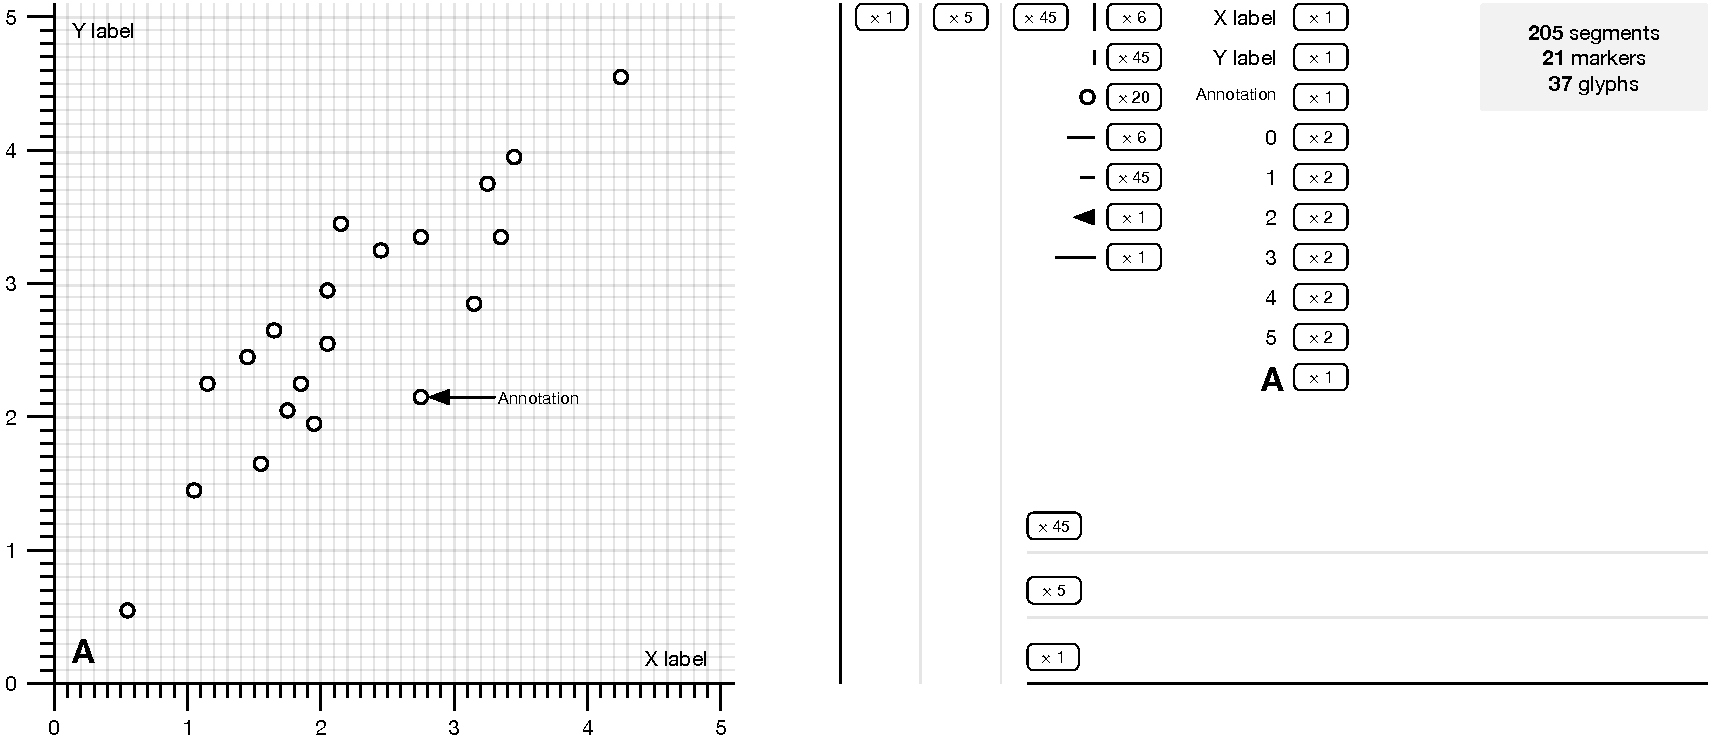
\includegraphics[width=0.92\textwidth]{legacy-plot-decomposition.pdf}
  \caption{A 2023 draft figure decomposing a scatter plot into elementary visual components. The
  figure remains useful, but the current \gsp framing treats these components as semantic visual
  families rather than as backend draw calls.}
  \label{fig:decomposition}
\end{figure}

That motivation remains correct, but the project has become more precise. The current \gsp design
is not merely a list of primitives. It is a session protocol with resources, visual families,
views, capabilities, queries, diagnostics, fixtures, and backend conformance evidence. The change is
important. A list of primitives risks becoming another graphics API. A protocol can define how
scientific visualization semantics survive across different renderers.

The 2023 draft also emphasized mutualization: a shared layer that lets libraries reuse work from
other libraries instead of rebuilding renderer engines. The current project keeps that aim but adds
three constraints that were less developed at the time:

\begin{itemize}
  \item Backend differences must be visible. A renderer must declare capabilities and return
  diagnostics when it simplifies, adapts, deactivates, or rejects a requested scene.
  \item Query and readback are not optional debugging features. They are part of the scientific
  visualization contract.
  \item Local performance matters. A protocol must allow a fast in-process path and must not force
  local GPU rendering through JSON or base64 serialization.
\end{itemize}

These constraints turn \gsp from a drawing vocabulary into a protocol architecture.

\section{What \gsp is not}

It is useful to define \gsp by exclusion before defining it positively.

\gsp is not a plotting API. It does not prescribe the user-facing experience of making a scatter
plot, an image viewer, a linked brushing tool, or a 3D mesh viewer. A plotting API can be concise,
stateful, declarative, grammar-based, notebook-oriented, or domain-specific. \gsp should be usable
under several such APIs.

\gsp is not a rendering engine. It does not require a specific rasterizer, GPU API, font system,
layout engine, window toolkit, or shader implementation. A \gsp renderer may be in-process,
subprocess-based, remote, browser-hosted, CPU-based, GPU-based, retained, immediate, or hybrid.

\gsp is not a file format. Debug JSON and conformance fixtures are useful, but they are not the
protocol itself. The protocol semantics should survive multiple encodings, including an in-process
Python path, binary IPC, network transport, and fixture/replay formats.

\gsp is not a promise that all renderers can do everything. Scientific visualization spans too many
output targets and hardware environments for that. The protocol instead requires explicit
capability discovery and explicit adaptation. This is closer to how robust systems are actually
built: know what the backend can do, plan against those facts, and do not silently degrade
scientific meaning.

\section{The protocol boundary}

The current \gsp architecture has four layers:

\begin{center}
\begin{tabularx}{0.92\textwidth}{@{}lX@{}}
\toprule
Layer & Role \\
\midrule
Producers & Plotting APIs, \vispytwo, domain viewers, notebooks, or application code that create
semantic scenes. \\
\gsp session and protocol & Backend-independent scene, resource, view, query, capability, and
diagnostic model. \\
Backend adapters & Translation from \gsp semantics to a concrete renderer's objects, commands,
state updates, and readback mechanisms. \\
Renderers & \matplotlib, \datoviz, remote renderers, browser renderers, or specialized scientific
rendering engines. \\
\bottomrule
\end{tabularx}
\end{center}

The protocol is organized around a session between a producer/client and a renderer/server. The
server may live in the same process, in a subprocess, on a remote machine, in a browser worker, or
behind a cloud service. It exposes capabilities, accepts resources and visual descriptions, executes
frames, returns query/readback results, and reports diagnostics. This framing is deliberately
inspired by successful protocol layers such as the Language Server Protocol: the important idea is
not a particular encoding, but a durable boundary between producers and implementations.

\begin{figure}[htbp]
  \centering
  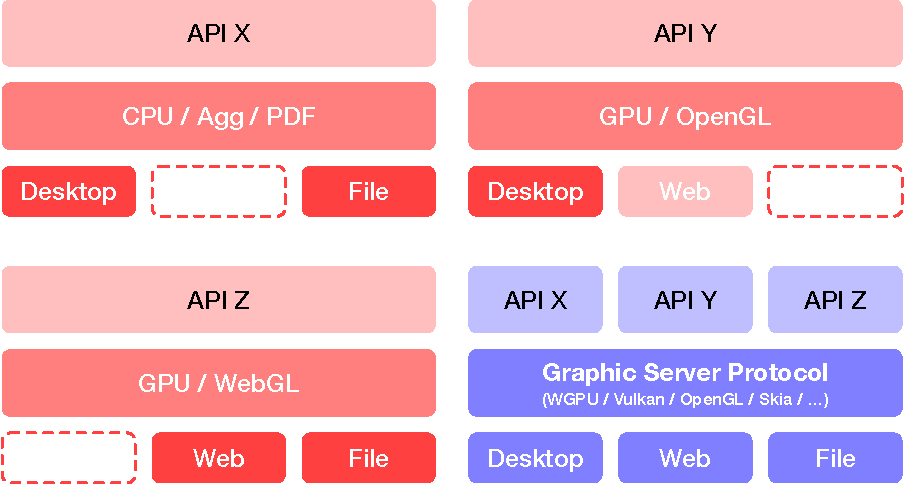
\includegraphics[width=0.9\textwidth]{legacy-gsp-architecture.pdf}
  \caption{The original 2023 architectural idea: multiple visualization APIs target an intermediate
  rendering protocol rather than binding directly to incompatible rendering engines. The current
  project keeps this structure but adds capability discovery, conformance, query/readback, and
  transport independence.}
  \label{fig:gsp-architecture}
\end{figure}

\subsection{Control plane and data plane}

\gsp separates the control plane from the data plane.

The control plane includes session initialization, capability negotiation, scene and visual updates,
view and navigation state, transforms, frame submission, query requests, diagnostics, and events.
These objects are relatively small and structured. They are the natural domain of schemas, versioned
fixtures, debug JSON, and protocol logs.

The data plane includes buffers, textures, tiles, chunks, sampled fields, external source handles,
cache policy, and level-of-detail descriptors. These objects may be large and should not be forced
through text encodings in local workflows. A local desktop renderer should be able to receive
NumPy-backed memory, direct buffers, or backend-native resources without paying a serialization tax.
A remote renderer may instead receive descriptors that let the server fetch or materialize data
under explicit security policy.

This split matters because scientific visualization commonly operates at the boundary where data is
too large to copy casually, but interaction still requires low latency.

\subsection{Transport independence}

The protocol semantics should not depend on one transport. Current design discussions distinguish
at least four transport classes:

\begin{itemize}
  \item in-process transport for fast local rendering;
  \item binary IPC or shared memory for local process boundaries;
  \item network transport for remote rendering or server-side data access;
  \item debug JSON for fixtures, replay, logging, and conformance tests.
\end{itemize}

This is a practical compromise. JSON fixtures are invaluable for testing and communication. They
are not acceptable as the only path for high-performance local rendering. Conversely, an in-process
Python adapter is not a sufficient protocol story for remote or polyglot renderers. \gsp needs both.

\section{Semantic visual families}

The 2023 draft described primitives as dots, points, markers, segments, paths, glyphs, images,
meshes, and volumes. The current project uses the term visual family to emphasize that the protocol
contract is semantic, not merely graphical. A visual family defines the meaning of data fields,
coordinate spaces, screen-space units, color interpretation, ordering rules, query identity, and
backend adaptation behavior.

The current baseline includes the following families and cross-cutting concepts:

\begin{center}
\begin{tabularx}{0.95\textwidth}{@{}lX@{}}
\toprule
Family or concept & Protocol role \\
\midrule
Point and marker & Screen-sized circular or shaped items with positions, colors, stroke/fill
semantics, and item identity. \\
Segment and path & One-dimensional stroked geometry with screen-space widths and cap/join
semantics. \\
Image & Raster data placed into a scene, including scalar image interpretation and origin/extent
semantics. \\
Text & Public text as strings with placement, anchoring, rotation, and logical font size; glyph
atlases remain backend realization details. \\
Mesh & Indexed triangle geometry with bounded material/shading semantics and 2D/3D view
placement. \\
Color mapping & Shared scalar-to-color semantics, normalization, named color scales, and
colorbar guides. \\
Guides and layout & Axes, ticks, labels, titles, colorbars, and resolved layout snapshots. \\
Views and transforms & View2D, View3D, affine transforms, projection, navigation actions, and
query inverse payloads. \\
\bottomrule
\end{tabularx}
\end{center}

This list is intentionally narrower than the universe of possible graphics. The point is not to
expose every feature of every renderer. The point is to stabilize the families that recur across
scientific visualization and make their semantics testable.

A backend is free to realize a point as a shader program, a CPU rasterized collection, a vector
artist, a set of instanced quads, or a remote rendering command. What it must not do is silently
change the scientific meaning of the point. If requested sizes are in logical screen pixels, the
backend must preserve that meaning or report an adaptation. If scalar colors require a particular
normalization, the backend must apply it or reject the request. If query support is advertised, the
backend must return item identities and payloads that match the visual family contract.

\section{Capabilities and adaptation}

Scientific visualization libraries often hide backend differences until a user hits a failure mode:
a plot looks different, a field is ignored, an interaction is unavailable, a remote render path
silently drops a feature, or a GPU backend produces an image that cannot be queried. \gsp takes the
opposite position: backend differences are part of the protocol.

Every renderer reports a capability snapshot. Capabilities cover protocol versions, supported
visual families, resource limits, texture and buffer formats, transform placement, render target
formats, output/export support, query/readback support, layout guarantees, extension support, data
source policy, and security posture.

Planning a scene against a backend can then produce one of four outcomes:

\begin{center}
\begin{tabularx}{0.9\textwidth}{@{}lX@{}}
\toprule
Outcome & Meaning \\
\midrule
Accept & The backend claims strict support for the requested semantics. \\
Simplify with diagnostic & The backend can render a simpler but explicit version. \\
Deactivate with diagnostic & The backend can omit a requested component without failing the
entire scene, but only with a visible diagnostic. \\
Reject with fatal diagnostic & The requested behavior cannot be supported without violating the
contract. \\
\bottomrule
\end{tabularx}
\end{center}

This model is essential if \gsp is to be trusted. Without explicit adaptation, a protocol becomes a
wish list. With explicit adaptation, a renderer can be useful before it is complete, while still
being honest about what it did.

Capabilities also let \gsp avoid false portability. For example, a renderer may strictly support
point rendering but not point picking. It may support static 3D mesh rendering but not triangle
picking. It may render guides visually but lack resolved layout snapshots for guide queries. It may
support scalar images but not remote tiled data sources. These distinctions matter to library
authors and users.

\section{Query and readback}

In many graphics APIs, rendering is the main product and picking is an afterthought. Scientific
visualization cannot afford that split. Interaction, inspection, annotation, linked views, brushing,
tooltips, measurement, and debugging all require the inverse question:

\begin{quote}
What rendered scene contribution is under this panel coordinate, and what scientific data does it
represent?
\end{quote}

\gsp treats query/readback as first-class protocol behavior. A query result should be able to carry
visual identity, item/group/face/voxel/texel identity, coordinate-space information, source data
coordinates, displayed color, depth or ordering information, guide hits, and extension payloads
where applicable.

This is more than traditional color-buffer picking. The query contract must survive transforms,
views, layout, guides, scalar color mapping, remote data sources, and backend adaptation. If a 2D
view is panned and zoomed, a query should report through the accepted view snapshot. If a 3D ray is
computed from a camera and projection, the result should say which snapshot it used. If a guide tick
label is hit, a guide-scoped query should distinguish that from a data visual. If a backend cannot
provide these guarantees, it should not advertise them.

The result is a stronger relationship between rendering and interpretation. \gsp does not merely
ask a backend to draw. It asks the backend to participate in a scientific visualization session.

\section{Reference and flagship backends}

\gsp needs more than a specification. It needs concrete backends that exercise different parts of
the design space.

\subsection{\matplotlib: reference, conformance, and publication}

\matplotlib is the reference backend. That does not mean it is the fastest backend or the only
correct backend. It means that it is an excellent place to define conservative semantics, publication
output, layout behavior, and CPU-side query or readback paths.

The \matplotlib adapter is valuable precisely because it is not a GPU renderer. It can provide a
clear reference implementation for visual families, scalar color mapping, guides, layout snapshots,
2D transforms, navigation actions, and small-scene conformance. It can also produce PNG, PDF, and
SVG-style publication artifacts where appropriate. Backend-native \matplotlib artists remain
implementation details; the protocol contract is the \gsp scene and result model.

\subsection{\datoviz: high-performance GPU rendering}

\datoviz is the flagship high-performance GPU backend. It brings the project back to one of its
original motivations: high-quality, fast rendering of scientific primitives using modern graphics
hardware. The \datoviz v0.4 direction is especially important because its internal scene, panel,
visual, camera, query, and capability model is close in spirit to \gsp, while still remaining a
concrete renderer with its own API and constraints.

The \gsp-\datoviz relationship should be understood as an adapter relationship, not as identity.
\gsp must not expose \datoviz-native handles as protocol semantics. \datoviz may have native
controllers, draw states, shader paths, and internal resources, but \gsp speaks in terms of visual
families, views, resources, capabilities, and query payloads. Where \datoviz can provide strict
support, it should advertise it. Where it can only adapt, that adaptation should be explicit. Where
the binding or runtime does not expose enough evidence, support should remain unadvertised.

\subsection{\vispytwo: producer API}

\vispytwo is the high-level Python producer target. Its role is different from both \matplotlib and
\datoviz. It should give Python users a modern scientific visualization API that can produce \gsp
scenes. This keeps user ergonomics out of the protocol core. \vispytwo can offer convenience,
defaults, domain-friendly helpers, and interactive workflows while relying on \gsp for backend
planning and rendering.

This separation is a key design discipline. If every user-facing convenience becomes protocol
semantics, the protocol becomes too large and too unstable. If the protocol is too low-level, every
producer must rebuild the same semantic model. \vispytwo is where that balance can be explored for
Python without forcing it on all possible producers.

\section{Conformance as a design tool}

A protocol without conformance evidence is difficult to discuss. The current project therefore uses
fixtures, review packs, capability matrices, diagnostics, and backend audits as part of the design
process.

\begin{figure}[htbp]
  \centering
  \begin{tabular}{cc}
    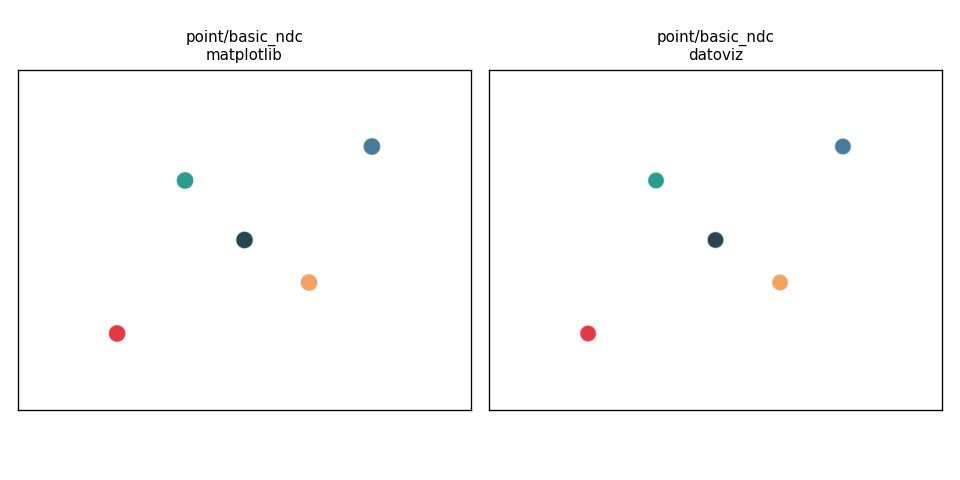
\includegraphics[width=0.45\textwidth]{review-point-basic.png} &
    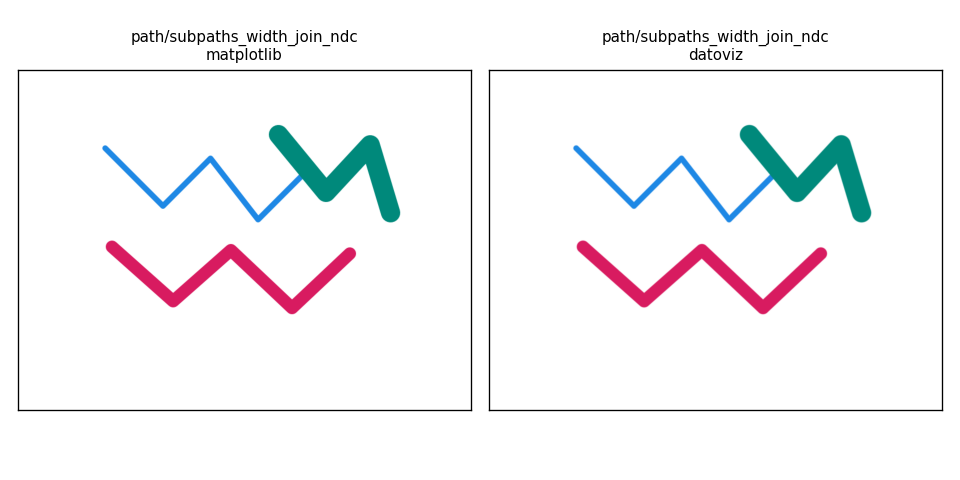
\includegraphics[width=0.45\textwidth]{review-path-subpaths.png} \\
    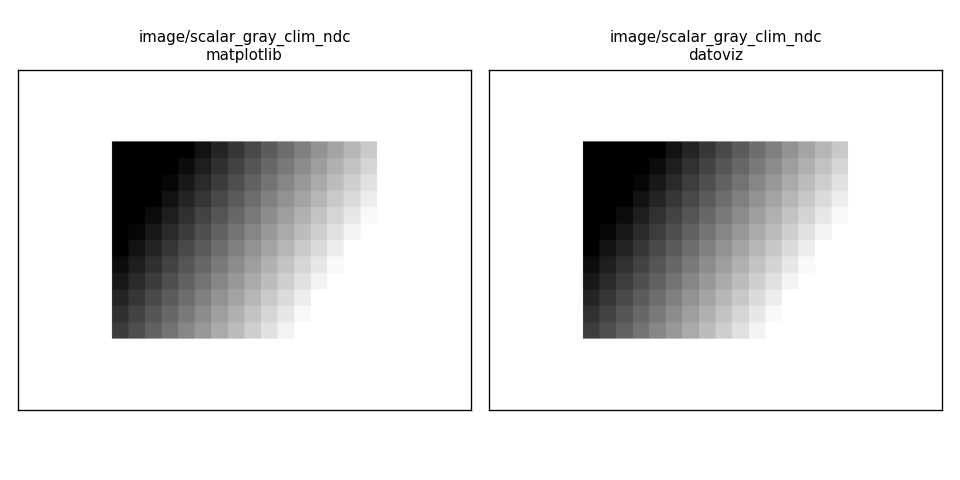
\includegraphics[width=0.45\textwidth]{review-image-scalar.png} &
    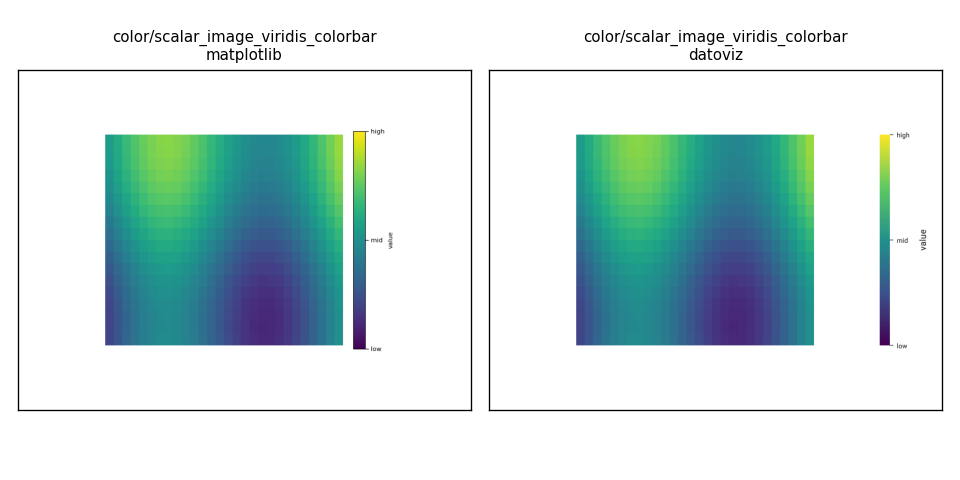
\includegraphics[width=0.45\textwidth]{review-colorbar.png} \\
    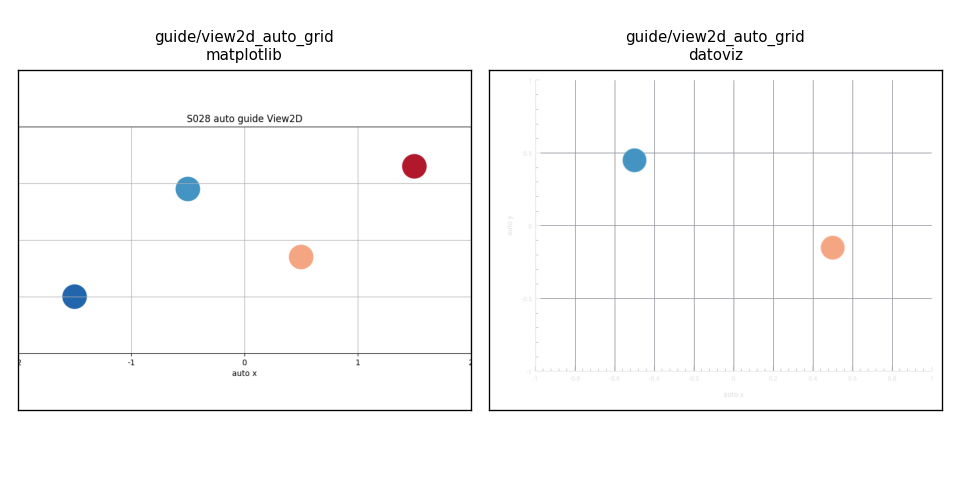
\includegraphics[width=0.45\textwidth]{review-guide-auto-grid.png} &
    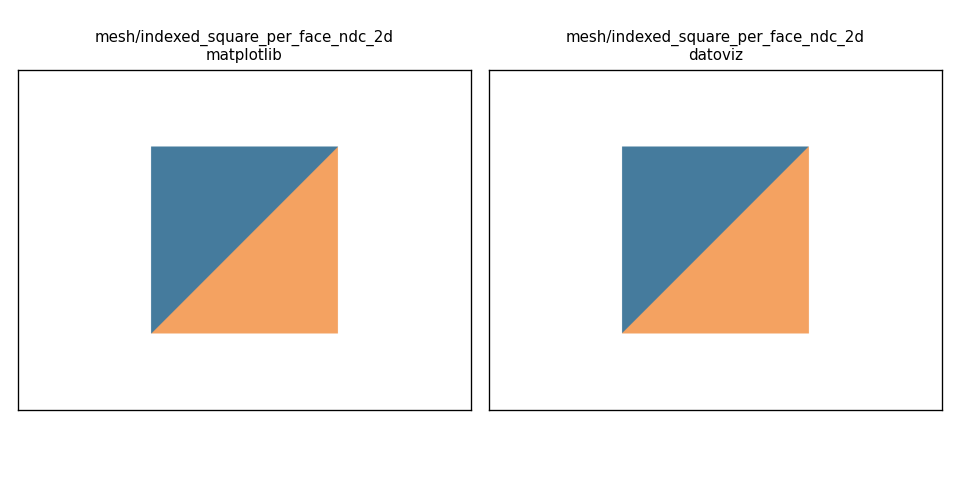
\includegraphics[width=0.45\textwidth]{review-mesh-per-face.png}
  \end{tabular}
  \caption{Representative visual review panels from the current implementation work: points,
  paths, scalar images, color mapping, guides, and meshes. Review packs are not a substitute for
  formal tests, but they make backend behavior visible across visual families and backends.}
  \label{fig:review-pack}
\end{figure}

The conformance strategy has several layers:

\begin{itemize}
  \item protocol fixtures that describe scenes and expected semantics;
  \item backend capability snapshots that state what is claimed;
  \item visual review packs that compare rendered outputs across backends;
  \item structured diagnostics for unsupported or adapted behavior;
  \item query/readback fixtures where interpretation matters;
  \item accepted design decisions and ADRs for changes that affect public semantics.
\end{itemize}

This process is deliberately conservative. A backend should not claim a capability simply because
an image looks plausible. Strict support requires matching the semantic contract and, where relevant,
matching query/readback behavior. A visually similar guide axis is not the same as resolved layout
strictness. A rendered 3D mesh is not the same as proven depth semantics and triangle picking. A
GPU path that displays text is not necessarily strict text semantics if anchoring, layout, query, or
font metrics are not yet covered.

For a community protocol, this discipline is not bureaucratic. It is what makes collaboration
possible. Different projects can implement different subsets while still speaking honestly about
their support.

\section{Large data, extensions, and remote rendering}

Large scientific data should not be treated as ordinary arrays once it exceeds the scale of local
eager rendering. Images may be tiled, volumes may be chunked, meshes may have levels of detail, and
data may live behind preconfigured sources or remote services. A protocol that assumes every visual
field is an eager client-side buffer will fail at exactly the scale where scientific visualization
becomes most important.

\gsp therefore reserves space for virtual data sources, extension manifests, source locality,
server-side fetch descriptors, decoder policy, cache policy, credential policy, and progressive
refinement. The current conservative posture is intentionally security-conscious: no dynamic
extension execution, no arbitrary network egress, no inline secrets, no unbounded materialization,
and explicit diagnostics for rejected sources or policies.

Extensions are necessary because no core protocol can anticipate every domain. A microscopy viewer,
geospatial viewer, connectomics tool, finite-element mesh viewer, or astronomical data cube may need
custom data sources, transforms, visual families, or query payloads. But extensions should not be
unstructured escape hatches. They need identifiers, versions, schemas, capability requirements,
fallback policy, implementation declarations, and query contracts.

This is one of the places where \gsp is intentionally more protocol-like than library-like. A library
can add a Python callback and trust the local process. A protocol must say what crosses the
boundary, what is safe to execute, what can be cached, what can be fetched, and how failures are
reported.

\section{Current status}

The current implementation is still a research and protocol-development effort, but it is no longer
only an idea. The repository now contains a substantial set of accepted specs, ADRs, protocol
models, backend adapters, fixtures, review packs, examples, and mission closeouts.

At a high level, the implemented/proven surface includes:

\begin{itemize}
  \item protocol-owned models for capabilities, command batches, resources, visual families,
  transforms, views, queries, diagnostics, and fixtures;
  \item visual family coverage for points, markers, segments, paths, images, text, and meshes;
  \item scalar color mapping and colorbar guide semantics;
  \item deterministic View2D navigation and layout-aware guide behavior;
  \item static View3D, orthographic and perspective camera work, and View3D navigation review paths;
  \item \matplotlib reference rendering for the core semantic families;
  \item \datoviz v0.4 adapter work for strict or adapted GPU rendering across many visual families;
  \item visual QA harnesses, contact sheets, backend capability matrices, and review examples;
  \item early extension and virtual data-source architecture with conservative security policy.
\end{itemize}

Equally important, some things remain explicitly not claimed:

\begin{itemize}
  \item \datoviz support is capability-gated where binding or runtime evidence is incomplete;
  \item some \datoviz guide/layout behavior remains adapted rather than strict;
  \item public volume and surface visual families remain future work;
  \item broad material, lighting, texture, and shader extension models remain deliberately bounded;
  \item native \datoviz mesh triangle picking is not advertised until public visual/primitive
  mapping and freshness are proven;
  \item governance, release process, and cross-project adoption are still open.
\end{itemize}

This status should be read as a strength rather than a weakness. A protocol proposal becomes more
credible when it distinguishes working semantics from aspirations.

\section{Relation to existing systems}

\gsp overlaps with several existing ideas, but it occupies a specific boundary.

\matplotlib backends separate a plotting API from output renderers, but within the \matplotlib
artist and figure model. \gsp asks whether a protocol layer can sit below multiple scientific
visualization APIs, not only one.

Vega and Vega-Lite demonstrate the power of declarative visualization specifications, especially in
browser contexts. \gsp is lower level and more renderer-oriented. It is not a grammar for charts; it
is a protocol for semantic visual scene execution, including local GPU paths and query/readback.

VTK and similar systems provide extensive scientific visualization capabilities, especially for 3D,
meshes, and volumes. \gsp is not a replacement for a large visualization toolkit. It is a protocol
surface that could, in principle, target or interoperate with such renderers for suitable subsets.

ANARI is a relevant comparison for 3D scientific rendering interoperability. \gsp is broader in the
sense that it targets 2D and 3D scientific visualization, guides, views, query semantics, and
producer/backend separation for plotting-like systems. It is narrower in other ways: it is not a
general physically based rendering API.

Browser graphics stacks, WebGPU, WebGL, Canvas, SVG, and WebAssembly provide important execution
targets. \gsp should be able to target browser renderers, but it should not be defined by browser
constraints alone. Scientific desktop use still needs a fast local in-process path.

\section{Community shape}

The long-term value of \gsp depends on whether it becomes a shared boundary rather than a private
implementation detail. That suggests several community goals:

\begin{itemize}
  \item keep the core protocol small enough to implement;
  \item define extensions for specialized domains instead of bloating the core;
  \item maintain conformance fixtures and capability vocabularies as public artifacts;
  \item make unsupported behavior explicit and testable;
  \item invite backend authors to implement subsets without requiring all features;
  \item invite plotting and domain-library authors to produce \gsp scenes without adopting one
  prescribed user API;
  \item separate governance of protocol semantics from any single renderer implementation.
\end{itemize}

The right governance model is still open. A lightweight consortium, a specification repository,
versioned extension registry, or working group around scientific visualization interoperability are
all plausible. What matters first is a clear protocol thesis and a credible proof that the boundary
can work.

\section{Conclusion}

Scientific visualization needs both diversity and reuse. It benefits from many user APIs, many
domain tools, many renderer implementations, and many deployment targets. But it pays a high cost
when every project has to rediscover the same renderer-facing semantics in isolation.

\gsp proposes a shared layer: not a plotting API, not a renderer, not a file format, but a semantic
graphics server protocol for scientific visualization. Its core ideas are straightforward:
describe visual scenes in backend-independent terms; discover capabilities before rendering;
adapt or reject explicitly; treat query/readback as part of the scientific contract; preserve a fast
local path; and use conformance evidence to make claims testable.

The current implementation work around \matplotlib, \datoviz, and \vispytwo suggests that this
boundary is practical. It is not finished. It is now concrete enough to discuss with the wider
scientific visualization community.

\section*{Selected references and related projects}

\begin{itemize}
  \item John D. Hunter. Matplotlib: A 2D graphics environment. \textit{Computing in Science and
  Engineering}, 2007.
  \item Nicolas P. Rougier. Shader-based antialiased 2D graphics and scientific visualization
  primitives, project notes and publications.
  \item Cyrille Rossant. Datoviz: Vulkan-based scientific visualization.
  \item Jeffrey Heer, Arvind Satyanarayan, and collaborators. Vega and Vega-Lite.
  \item Khronos Group. ANARI: Analytic Rendering Interface.
  \item Microsoft and contributors. Language Server Protocol.
  \item The Visualization Toolkit (VTK).
\end{itemize}

\end{document}
